%\documentclass[twoside,11pt]{article}
\documentclass[11pt]{article}
\usepackage[natbib, preprint]{jmlr2e}

\usepackage{enumitem}
\usepackage{amsmath}
\usepackage{color}
\usepackage[toc,page]{appendix}
\usepackage{amssymb}
\usepackage{graphicx}
\usepackage{epstopdf}
\usepackage{hyperref}
\usepackage{alltt}
\usepackage{listings}
\usepackage{array}
\usepackage[noline, boxed, linesnumbered, procnumbered, titlenumbered]{algorithm2e}
\usepackage{caption}
\usepackage{subcaption}


\newcommand{\secref}[1]{Section~\ref{#1}}
\newcommand{\appdxref}[1]{Appendix~\ref{#1}}
\newcommand{\tblref}[1]{Table~\ref{#1}}
\newcommand{\figref}[1]{Figure~\ref{#1}}
\newcommand{\thmref}[1]{Theorem~\ref{#1}}
\newcommand{\algref}[1]{Algorithm~\ref{#1}}
\newcommand{\funref}[1]{Function~\ref{#1}}
\newcommand{\eqnref}[1]{Equation~\ref{#1}}
\newcommand{\listingref}[1]{Listing~\ref{#1}}

\newcommand{\eg}{{\em e.g.}}
\newcommand{\ith}{$i^{th}$}
\newcommand{\cut}[1]{}
\newcommand{\todo}[1]{{{\color{red}{[#1]}}}}

\newcommand{\Ex}{\mathop{\mathbb{E}}}
%\newcommand{\Imp}{\mathbf{I}}
\newcommand{\Imp}{\text{Impact}}

\newcommand{\simp}{\fontfamily{cmr}\textsc{\small StratImpact}}
\newcommand{\spd}{\fontfamily{cmr}\textsc{\small StratPD}}
\newcommand{\cspd}{\fontfamily{cmr}\textsc{\small CatStratPD}}
\newcommand{\xnc}{$x_{\overline{c}}$}
\renewcommand{\xi}{x^{(i)}}
\newcommand{\xnC}{$x_{\overline{C}}$}

\setlist[enumerate]{itemsep=-1mm}

% DON'T change margins - should be 1 inch all around.
\cut{
\addtolength{\oddsidemargin}{-.5in}%
\addtolength{\evensidemargin}{-.5in}%
\addtolength{\textwidth}{1in}%
\addtolength{\textheight}{1.3in}%
\addtolength{\topmargin}{-.8in}%
}

\ShortHeadings{Tech Report: Model-Free Feature Importance}{Parr, Wilson, and Hamrick}
\firstpageno{1}

\begin{document}

\def\spacingset#1{\renewcommand{\baselinestretch}%
{#1}\small\normalsize} \spacingset{1}


%%%%%%%%%%%%%%%%%%%%%%%%%%%%%%%%%%%%%%%%%%%%%%%%%%%%%%%%%%%%%%%%%%%%%%%%%%%%%%

\title{\bf Tech Report: Model-Free Feature Importance}

\author{Terence Parr \email parrt@cs.usfca.edu
\addr University of San Francisco\\
\AND James D. Wilson \email jdwilson4@usfca.edu
\addr University of San Francisco\\
\AND Jeff Hamrick \email jhamrick@usfca.edu
      \addr University of San Francisco}

\maketitle

\begin{abstract}%
awesome abstract here
\end{abstract}

\begin{keywords}
feature importance, business insights, medical insights, partial dependence, model interpretability, machine learning
\end{keywords}

\section{Introduction}
\label{sec:intro}

Among data analysis techniques, feature importance is one of the most useful and is used by practitioners for two key purposes. First, to select features for predictive models (dropping the least predictive features to simplify and potentially increase the generality of the model). Second, to gain business or medical insights, such as identifying product characteristics valued by customers or treatments contributing to patient recovery.  To distinguish the two use cases, we will refer to feature predictiveness for modeling purposes as {\em importance} (the usual meaning) and the effect of features on business or medical response variables as {\em impact}.

While some feature importance approaches work directly on the data, such as minimal-redundancy-maximal-relevance (mRMR) by \cite{mRMR}, almost all algorithms used in practice rank features by interrogating a specific fitted model (e.g., SHAP \citep{shap}), permutation importance \citep{RF}, and drop column importance), or even interrogating subsidiary models to analyze such fitted models (e.g., LIME \citealt{lime}). It is accepted as self-evident that identifying the most important features for a model is through interrogation of that  model, but this is not always the case.  For example, when asked to identify the single most important feature of a real dataset (\citep{bulldozer}), through interrogation and validation on a random forest, the features selected by model-based techniques get twice the validation error of the model-free technique proposed in this paper (\figref{fig:topk}(c)). Still, model interrogation is generally effective in practice for feature importance purposes. (In our experience, it is best to get importances using multiple techniques and to view the combined results as a clue rather than the gospel truth.)

Feature importance should not, however, be interpreted as feature impact for several reasons. First, predictive features do not always coincide with impactful features; e.g., models unable to capture complex nonlinear feature-response relationships rank such features as unimportant, even if they have large impacts on the response. Next, practitioners must develop models accurate enough to yield meaningful feature importances, but there is no definition of ``accurate enough.'' Finally, it is possible to get very different feature importances (and hence impacts) running the same algorithm on the same data, just by choosing a different model. This is despite the fact that true feature impacts are relationships that exist in the data, with or without a model.

Consider the feature importance charts in \figref{fig:diff-models} derived from four different models on the same, well-known Boston toy data set, as computed by SHAP that has recently emerged as the front runner in feature importance. The linear model (a) struggles to capture the relationship between features and target ($R^2$=0.74), so those importances are less trustworthy.  In contrast, the random forest (b), boosted trees (c), and support vector machine (d) models capture the relationship in the training records (all 506) with high fidelity, but SHAP derives meaningfully different feature importances from each model. The differences arise because feature importances are distorted by the lens' of the models, making it unclear which ranking, if any, gives the true feature impacts. 

\begin{figure}[htbp]
\begin{center}
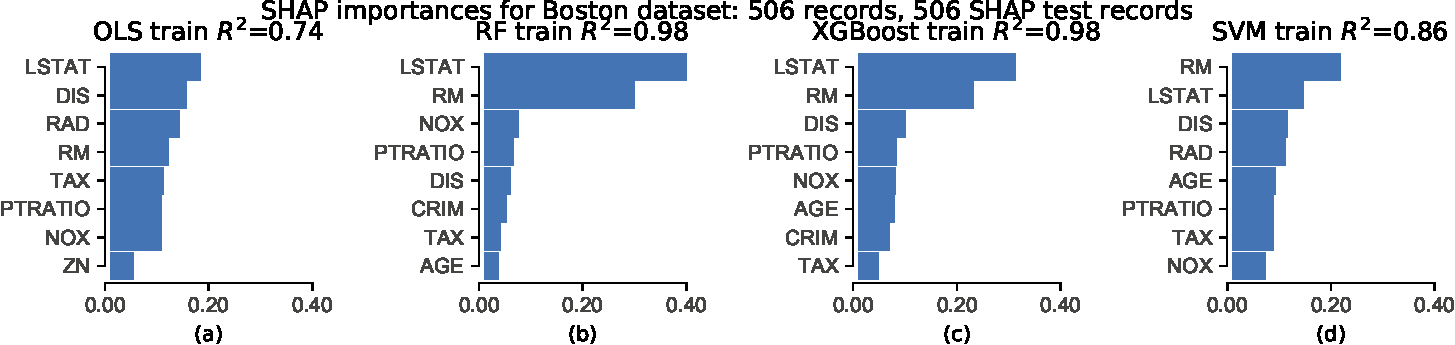
\includegraphics[scale=0.6]{images/diff-models.pdf}
\caption{Top 8 of 13 features. {\tt\footnotesize RandomForestRegressor(n\_estimators=30)}, {\tt\footnotesize XGBRegressor(max\_depth=5, eta=0.01, n\_estimators=50)}, {\tt\footnotesize SVR(gamma=0.001, C=100)} High var for RF. nshap=n test records. Rough timing for explaining 506 test records is (a) less than 1 second, (b) 10s, (c) 3s, and (d) 13 minutes.}
\label{fig:diff-models}
\end{center}
\end{figure}

Unfortunately, practitioners routinely conflate feature importance with impact and have, consequently, likely made business or medical decisions based upon faulty information. Despite the potentially serious real-world consequences resulting from inappropriate application of importances, research attention has focused primarily on feature importance rather than impact. 

In this paper, we address this deficiency by contributing (1) a simple mathematical formula for computing feature impact that is purely a function of the training data, rather than a fitted model  provided by the user, and (2) an efficient implementation called \simp{} that yields plausible feature impacts.   In order to measure the quality of feature impacts, we observe that features with the most impact on the response variable should coincide with the most predictive features, particularly if variable density among the validation records is taken into consideration. We, therefore, define feature importance as a weighted variation of feature impact. Using impact-derived importances as a proxy for impacts, our experiments on real data show that \simp{} is competitive with existing importance techniques, as measured by cross-validation errors on models trained using the top importances.   We emphasize that these impact and importance definitions are insensitive to codependencies among features and apply to both numerical and categorical features.  (The latter is essential because virtually all real-world datasets have categorical variables.) While we focus solely on regression here, a similar approach would work for classification.

We begin by giving definitions of feature impact and importance in \secref{sec:def}, then survey  existing model-free and model-dependent techniques in \secref{sec:existing}. \secref{sec:experiments} compares \simp{} to ... \todo{finish walkthrough}

\section{The definition of feature impact}\label{sec:def}

\cut{Practitioners loosely define feature importance as feature predictiveness, which presupposes a fitted predictive model, probably because importances are so often used for feature selection during model development.  Research  focuses on more accurately identifying the impact of features upon model predictions.  But, relying on a fitted model makes it difficult to tease apart the true feature importance from the ability of the model to exploit that feature for prediction purposes. Rather than measuring feature impact on {\em model predictions}, we propose avoiding the model completely to define feature importance as the average impact of a feature on the {\em data set response values}.}

In special circumstances, we know the precise impact of each feature $x_j$. Assume we are given training data pair ($\bf X, y$) where ${\bf X} = [x^{(1)}, \ldots, x^{(n)}]$ is an $n \times p$ matrix whose $p$ columns represent observed features and ${\bf y}$ is the $n \times 1$ vector of responses.  If a data set is generated using a linear function, $y = \beta_0 + \sum_{j=1}^p \beta_j x_j$, \todo{assumes independence of $x_j$?} then coefficient $\beta_j$ corresponds exactly to the impact of $x_j$.  $\beta_j$ is the impact on $y$ for a unit change in $x_j$, holding all other features constant.

To hold features constant for any smooth generator function, we can take the partial derivatives of $y$ with respect to each feature $x_j$. For any smooth function $f:\mathbb{R}^{p} \rightarrow \mathbb{R}$ that precisely maps each $\xi$ to $y_i$, ${y_i} = f(\xi)$, \todo{should that be $y^{(i)}$ to be consistent?} the partial derivative of $y$ with respect to $x_j$ gives the change in $y$ holding all other variables constant; e.g., for linear functions, $\frac{\partial y}{\partial x_j}=\beta_j$. Integrating the partial derivative then gives the {\em partial dependence}  of $y$ on $x_j$, the isolated contribution of $x_j$ to $y$. But, rather than relying on a fitted model as originally formulated by \citep{PDP}, this definition of partial dependence relies on the partial derivative of a known function that generated the data set.

~\\
\noindent {\bf Definition 1} The {\em model-free partial dependence} of $y$ on feature $x_j$ for smooth generator function $f:\mathbb{R}^{p} \rightarrow \mathbb{R}$ evaluated at $x_j = z$ is the cumulative sum up to $z$:

\begin{equation}\label{eq:pd}
\text{\it PD}_j(z) = \int_{min(x_j)}^z \frac{\partial y}{\partial x_j} dx_j
\end{equation}

$\text{\it PD}_j(z)$ is the value contributed to $y$ by $x_j$ at $x_j = z$. The advantages of this partial dependence definition are that it does not depend on a fitted model and is insensitive to collinear or otherwise codependent features, unlike the traditional definition that is accurate for data ``{\em dominated by low order interactions}'' per Friedman.  

To go from partial dependence to feature impact, we compare the area under the absolute value of each partial dependence curve. The larger the area under the curve, the larger the impact on $y$.   By the mean-value theorem of integrals, the area under $f(x)$ in interval $[a,b]$ is $\int_{a}^{b} f(x) dx = \overline{f(x)}(b-a)$.  For comparison purposes between variables, the actual area is not important and the $b-a$ term drops out, assuming the variables our normalized so all $x_j$ domains have the same range, such as $[0,1]$. The impact of $x_j$ is then just the average magnitude of $\text{\it PD}_j(x_j)$:

~\\
\noindent {\bf Definition 2} The feature impact, $\Imp_j$, of $x_j$ is the ratio of $x_j$'s average partial dependence magnitude to the total of all variables, when all $x_j$ variables are normalized to the same fixed range:

\begin{equation}\label{eq:Epd2a}
\Imp_j = \frac{\overline{|\text{\it PD}_j|}}{\sum_{k=1}^p \overline{|\text{\it PD}_k|}}
\end{equation}

\noindent For example, consider quadratic equation $y = x_1^2 + x_2 + 100$ as a generator of data in $[0,3]$. The partial derivatives are $\frac{\partial y}{\partial x_1} = 2 x_1$ and $\frac{\partial y}{\partial x_2} = 1$, giving $\text{\it PD}_1 = x_1^2$ and $\text{\it PD}_2 = x_2$. The areas under the partial dependence curves in $[0,3]$ are $\Imp_1 = \frac{x_1^3}{3} \big |_0^3 = 9$ and $\Imp_2 = \frac{x_2^2}{2} \big |_0^3 = 4.5$.   Therefore, $x_1$ has twice the impact as $x_2$ for data generated in that interval with impacts $\Imp_1 = 0.\overline{66}$ and $\Imp_2 = 0.\overline{33}$. \figref{fig:quad-area} shows...


\begin{figure}[htbp]
\begin{center}
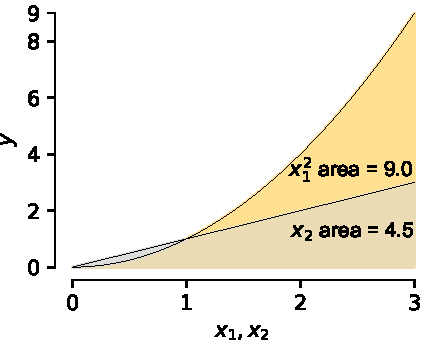
\includegraphics[scale=0.6]{images/quadratic-auc.pdf}
\captionof{figure}{\small $\Imp_1$, $\Imp_2$ for partial dependence curves from $y = x_1^2 + x_2 + 100$ in $[0,3]$}
\label{fig:quad-area}
\end{center}
\end{figure}

The obvious disadvantage of this feature impact definition is that function $f$, from which $\text{\it PD}_j$ is derived, is unknown in practice, so symbolically computing the partial derivatives is not possible. But, if we could compute accurate partial dependence curves by some other method, then this definition would still represent a viable means to obtain feature impacts. 

As originally defined, partial dependence curves are derived from fitted models and are biased in the presence of codependent variables.  To overcome this bias and to avoid the need for predictions from a fitted model, we recently introduced a technique called \spd{} (\citep{stratpd}) to approximate partial dependence curves using a data stratification approach. \spd{} stratifies a data set into groups of observations that are similar, except in the variable of interest, $x_j$, through the use of a single decision tree. Any fluctuation of the response variable within a group (decision tree leaf) is likely due to $x_j$. The $\beta_1$ coefficient of a simple local linear regression fit to the $(x_j, y)$ values within a group provides an estimate of $\frac{\partial y}{\partial x_j}$ in that group's $x_j$ range. Averaging the partial derivative estimates across all such groups yields the overall $\frac{\partial y}{\partial x_j}$ partial derivative approximation. The cumulative sum of the partial derivative yields the partial dependence curve. 

For categorical variables, \cspd{} uses the same stratification approach, but cannot apply  regression of $y$ on categorical $x_j$. Instead, a random reference category is chosen for each group and its $y$ value is subtracted from all leaf $y$ to get relative impacts between categories. The relative category impacts across groups are then averaged to get the impact of each $x_j$ on $y$.  (Note that \cspd{} and \spd{} never use predictions from any model---they use decision trees merely to stratify feature space and \spd{} uses piecewise linear regressors just to get slope estimates.)

\begin{figure}[htbp]
\begin{center}
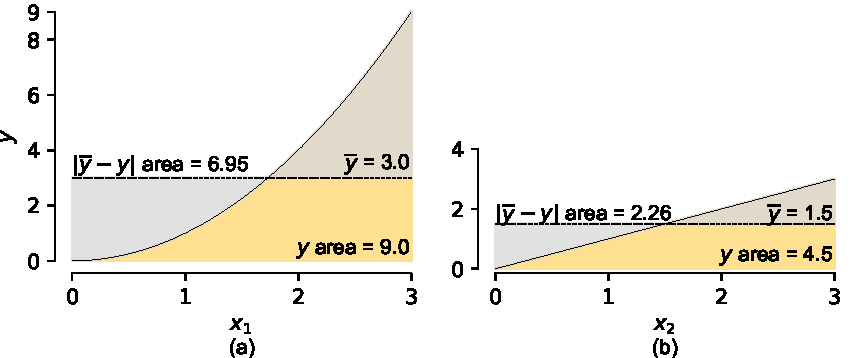
\includegraphics[scale=0.65]{images/from-mean-auc.pdf}
\captionof{figure}{AUC for partial dependence curves from $y = x_1^2 + x_2 + 100$ in $[0,3]$ Shows why must compute from 0 not deviation from mean}
\label{fig:combined-area}
\end{center}
\end{figure}

Intuitively, the impact of $x_j$ is how much, on average, the values of $x_j$ are expected to push $y$ away from zero. We deliberately chose this  definition instead of measuring how much $x_j$ pushes $y$ away from the average response, $\overline{y}$. The impact of $x_1$ on $y$ is $x_1^2$, not $\overline{y} - x_1^2$; e.g., at $x_j=0$, the impact on $y$ should be 0, not $\overline{y}-0 = \overline{y}$.  \figref{fig:combined-area} illustrates how the area under the $x_1^2$ and $x_2$ partial dependence curves from $y = x_1^2+x_2+100$ differ from the area straddling the means. The true area under the curve ratio of $x_1$-to-$x_2$ is 2-to-1 (9/4.5), whereas the ratio of the area straddling the mean has roughly a 3-to-1 ratio (6.95/2.26). \todo{is this clear enough?}

\begin{figure}[htbp]
\begin{center}
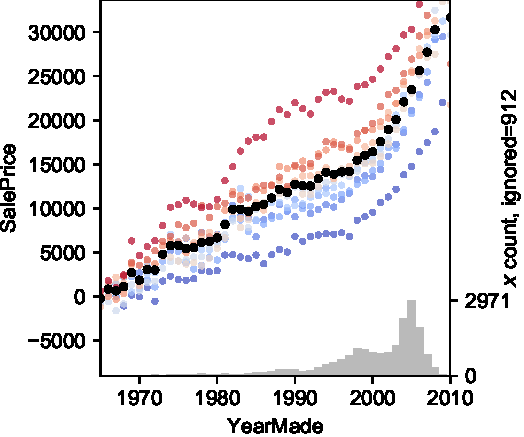
\includegraphics[scale=0.5]{images/bulldozer-YearMade.pdf}
\captionof{figure}{\small AUC for bulldozer features weighted by evidence, 20, 000 records of 401,125}
\label{fig:yearmade}
\end{center}
\end{figure}

For business or medical insight purposes, deriving feature impacts from partial dependence curves make sense because these curves describe how each $x_j$ value found in the data set effects $y$. When selecting features for modeling, however, feature impact values should take $x_j$ density into consideration. Model validation error is sensitive to the distribution of the records in the validation set, not just the selection of most impactful features.  For example, \figref{fig:yearmade} shows the partial dependence curve for feature {\tt\small YearMade} and the histogram of $x_j$ values from the bulldozer auction data set \citep{bulldozer}; the colored curves represent ten bootstrapped data sets and the black dots give the average curve.  Knowing that increased bulldozer age continues to reduce price is useful from a business perspective, but the bulk of the validation set will have newer bulldozers.  This leads to a feature importance definition based upon expected value of the partial dependence magnitude rather than simple averages across $x_j$ domains.

\cut{
While feature importances should not be interpreted as feature impacts, impacts can be effective as feature importances for model feature selection.  Features with the most impact on the response variable the most should coincide with the most predictive features. But, m

The definition of impact in \eqnref{eq:Epd2a} assumes that each $x_j$ value is equally likely, which is not the case in practice for $(\bf X, y)$ data sets. To go from partial dependence to importance, the $\text{\it PD}_j$ curve at $x_j=z$ must be weighted by the number of samples at $x_j=z$ before computing the average magnitude.  The red dots represent the $\text{\it PD}_j$ weighted according to the histogram height and the orange region represents the impact {\tt\small YearMade} has on target {\tt\small SalePrice}. While the {\tt\small YearMade} partial dependence curve is plausible before year 1990 (older bulldozers are worth less), there are so few data points that the collection of very old bulldozers should have little overall effect on the overall average sale price.  This leads to a definition based upon expected value rather than simple averages across $x_j$ domains.
}

~\\
\noindent {\bf Definition 3} The {\em model-free feature importance}, $\text{Impo}_j$, of $x_j$ is the ratio of $x_j$'s expected partial dependence value to the total of all expected values, when all $x_j$ variables are normalized to the same fixed range:

\begin{equation}\label{eq:Epd2b}
\text{Impo}_j = \frac{\Ex[|\text{\it PD}_j|]}{\sum_{k=1}^p \Ex[|\text{\it PD}_k|]}
\end{equation}

\noindent where:

\begin{equation}\label{eq:Epd2c}
\Ex[|\text{\it PD}_j|] = \frac{1}{n} \sum_{i=1}^{n} |x_j[x_j=x_j^{(i)}]| \times  |\text{\it PD}_j(x_j^{(i)})|
\end{equation}

\noindent and $x_j[x_j=x_j^{(i)}]$ denotes the count of $x_j$ values equal to $x_j^{(i)}$.

\todo{ need something better than Impo... how should we denote impact and importance?}

\todo{
\begin{itemize}
\item Do we need to explain why that is a weighted sum? i.e., repeated $x_j^{(i)}$ values and in repeated partial dependence values.
\item in our case $n$ differs for each $x_j$ due to implementation details of \spd{} but in the general case can't we therefore remove that common factor and just say that the weighted sum relative to other variables' weighted sum is the importance?
\item do we need to point out that $\sum_{k=1}^p \Ex[|\text{\it PD}_k|]$ is not the expected value of avg $|y|$? I.e., why are we not dividing by avg $|y|$?
\end{itemize}
}

 
\section{Existing methods}\label{sec:existing}

In this paper, we are primarily concerned with identifying the most impactful features for business or medical applications. But, because virtually all research focuses on feature importance and because practitioners commonly to assume feature importance is feature impact, it is appropriate to compare \simp{} to existing feature importance methods.

Feature importance methods for labeled data sets (with $\bf X$ and $\bf y$) are broadly categorized into data analysis and model analysis techniques, sometimes called {\em filter} and {\em wrapper} methods \citep{tsanas}. Data analysis techniques analyze the data directly to identify important features, whereas model analysis techniques rely on predictions from fitted models.  The intended application of the feature importances (business insight or feature selection) often dictates the approach.  The data analysis techniques further split into techniques for regression and techniques for classification, with most of the research going into classification.

The simplest technique to identify important or relevant regression features is to rank them by their Spearman's rank correlation coefficient \citep{spearmans}; the feature with the largest coefficient is taken to be the most important. This method works well for independent features, but suffers in the presence of codependent features.   Groups of features with similar relationships to the response variable receive the same or similar ranks, even though just one should be considered important.

Another possibility is to use principle component analysis (PCA), which operates on just the $\bf X$ explanatory matrix. PCA transforms data into a new space characterized by eigenvectors and identifies features that explain the most variance in the new space. If the first principal component covers a large percentage of the variance, the ``loads'' associated with that component can indicate importance of features in the original $\bf X$ space. PCA is limited to linear relationships, however, and ``most variation'' is not always the same thing as ``most important.''

For classification data sets, the Relief algorithm \citep{relief} tries to identify features that distinguish between classes through repeated sampling of the data. For a sampled observation $\xi$, the algorithm finds the nearest observation with the same class (hit) and the nearest observation with the other class (miss). The score of each attribute, $x_j$, is then updated according to the distance from the selected $\xi$ to the hit and miss observations'  $x_j$ values. ReliefF \citep{ReliefF} extended Relief to work on multiclass problems and RReliefF \citep{RReliefF} adapted the technique to regression problems (by ``...introduc[ing] a kind of probability that the predicted values of two instances are different'').

In an effort to deal with codependencies, data analysis techniques rank features not just by {\em relevance} (correlation with the response variable) but also by low {\em redundancy}, the amount of information shared between codependent features, which is the idea behind minimal-redundancy-maximal-relevance (mRMR) by \citep{mRMR}. mRMR selects features in order according to the following score.

\[
J_{mRMR}(x_k) = I(x_k, y) - \frac{1}{|S|} \sum_{x_k \in S} I(x_k, x_j)
\]

\noindent where $I(x_k, x_j)$ is some measure of mutual information between $x_k$ and $x_j$, $S$ is the growing set of selected features, and $x_k$ is the candidate feature. mRMR only considers single-feature relationships with the response variable, and is limited to classification as originally defined. See \citep{ubermRMR} for a recent application of mRMR at Uber Technologies.  For more on model-free feature importances, see the survey by \citep{survey}.  \citet{tsanas} suggests using spearman's rank not mutual information. \citet{meyer-microarray} looks for pairs of features to target associations as an improvement, while retaining reasonable efficiency. See \citet{filter-benchmark} for benchmarks of filter on filter methods.

The fundamental problem faced by all of these data analysis techniques is that they measure relevance by the strength of the association between (typically) a single feature to response $y$, but $y$ contains the impact of all $x_j$ variables. Computing an appropriate association metric between categorical and numeric values also presents a challenge.  In contrast, the definitions of impact and importance proposed in this paper isolate the effect of each $x_j$ on $y$, holding all other variables constant, and also support categorical features.
 
Turning to model-based techniques, feature importance methods are typically variations on a theme: tweak the model and measure the effect on model prediction accuracy or expected model output. The simplest approach is {\em drop-column importance}, which defines $x_j$ importance as the difference in model accuracy between a model with all features and a model with $x_j$ removed. The model must be retrained $p$ times and highly similar features yield low or zero importances because codependent features cover for the dropped column in the model.

To avoid retraining the model, $x_j$ can be permuted instead of dropped for {\em permutation importance}. This approach is faster but can introduce nonsensical observations by permuting invalid values into records; e.g., shifting a true {\tt\small pregnant} value into a male's record. Codependent features tend to share importance, at least when applied to random forest models.

Rather than removing or permuting entire columns of data, LIME \citep{lime} and SHAP \citep{shap} focus on model behavior at the observation level. For a feature vector of interest, LIME trains an interpretable linear model, on a small neighborhood of data around that vector to explain the relationship between variables and the response locally. SHAP, however, was shown to subsume the LIME technique in \citep{shap}.

SHAP has its roots in {\em Shapley regression values} \citep{shapley-regression} where (linear) models were trained on all possible subsets of features.  Each possible model pair differing in a single feature $x_j$ contributed the difference in model pair output towards the Shapley value for $x_j$. The complete Shapley value is the average model-pair difference weighted by the number of possible pairs differing in just $x_j$.  For completely independent features, drop-column importance is sufficient because the contribution of $x_j$ can be computed without considering how combinations of features affect model output.  In practice, features are rarely independent and the marginal effect of adding a new feature on model output depends on the order in which features are added.  

To avoid training a combinatorial explosion of models with the various feature subsets, SHAP reuses the same model by running simplified feature vectors into the model. Simplified vectors replace ``missing'' $x_j$ features with the expected value of $x_j$ \todo{isn't it $E[f(z)]$? hold on, they are approximating $f(z_S)$ not missing $x_j$ features; another description indicates that you replace missing values with a random one selected from other records}, to simulate models trained on feature subsets. To further reduce computation costs, SHAP users typically compute values for a small subsample of the data set. SHAP has model-type-dependent optimizations for linear regression, deep learning, and decision-tree based models. 

While SHAP has very strong theoretical foundations, we observed several disadvantages:

\begin{itemize}
\item  For performance reasons, SHAP limits the user's choice of model to those with model-type-dependent implementations, such as {\tt\small TreeExplainer}; e.g., SHAP applied to a support vector machine trained on Boston's 506 records takes 13 minutes to explain the same 506 records.  Large data sets also pose problems even for the model-type-dependent optimizations; e.g., SHAP applied to a modest 50-tree random forest trained on 1.2M record ``League of legends'' data set \citep{lol} takes 25 minutes to process sample of size 1000.

\item As with permutation methods, replacing feature values with their expectations \todo{or random sample?} introduces the possibility of creating nonsensical feature vectors.  For example, replacing the bulldozer {\tt\small YearMade} feature with the overall {\tt\small YearMade} average, risks conjuring up a type of bulldozer that did not exist in that year. This biases the feature contribution estimates.

\item SHAP documentation claims to break ``the dependencies between features according to the rules dictated by casual inference'' citing \citet{janzing2019feature}, but we find this SHAP ``interventional'' mode is still unable to disentangle codependent features for a synthetic body weight data set with codependent {\tt\small sex}/{\tt\small pregnant}/{\tt\small height} features from Equation (7) in \citet{stratpd}:

\begin{equation}\label{eq:weight}
y_{weight}  = 120 + 10(x_{height} - min(x_{height})) + 70x_{pregnant} - 1.5x_{education}
\end{equation}

\noindent with 50/50 male/female, half of the women are pregnant, and women gain an inflated 70 pounds to make the bias more prominent. \figref{fig:shap-weight}(a) illustrates the original SHAP partial dependence between height and weight and (b) shows that the interventional SHAP is improved but still biased by codependent features.  The exact partial dependence relationship between height and weight should be a line with slope 10, which is what \spd{} computes and draws on top of the SHAP plots in \figref{fig:shap-weight}; see \citet{stratpd} for more details.

\item  We cannot agree with the SHAP definition of feature importance, which measures the effect of features as they cause deviations from the mean model prediction. This definition effectively measures the area straddling the mean of the partial dependence curve rather than the area under the curve.  Revisiting \figref{fig:combined-area}, SHAP measures the gray area and \simp{} measures the orange area.  Given the associated generator function, $y=x_1^2 + x_2 + 100$, we know the partial dependence curves are $x_1^2$ and $x_2$.  By our definition, the impact is the area under $x_1^2$ and $x_2$, not the areas straddling the mean of $x_1^2$ and $x_2$. \todo{need to explain why they are wrong or is it obvious?} 

\item SHAP often gives plausible partial dependence curves, but we found several questionable cases for features identified as important. \figref{fig:shap-stratpd-YearMade} gives one such example, comparing the marginal plot of  bulldozer YearMade to SalePrice (a), SHAP partial dependence of SalePrice on YearMade (b), and \spd{}'s curve (c). The SHAP does not show the expected relationship, that of decreased value for older bulldozers.

\end{itemize}

\begin{figure}[htbp]
\begin{center}
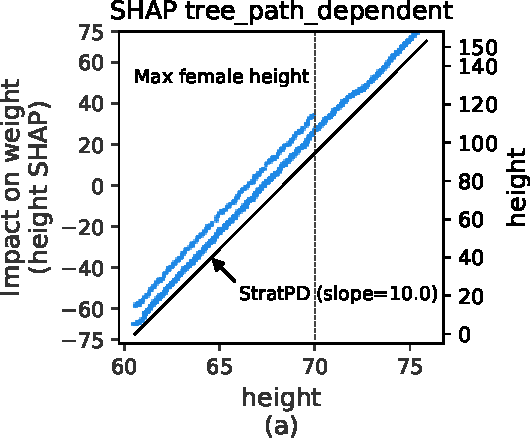
\includegraphics[scale=0.5]{images/weight-shap-tree_path_dependent.pdf}~~
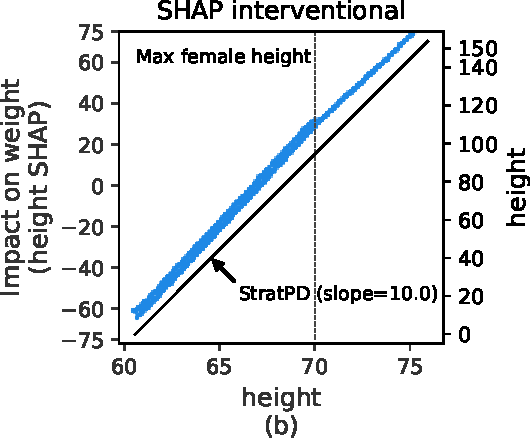
\includegraphics[scale=0.5]{images/weight-shap-interventional.pdf}
\caption{\small Plots of height versus body weight using 2000 observations from Equation \eqref{eq:weight} as drawn by SHAP library}
\label{fig:shap-weight}
\end{center}
\end{figure}

\begin{figure}[htbp]
\begin{center}
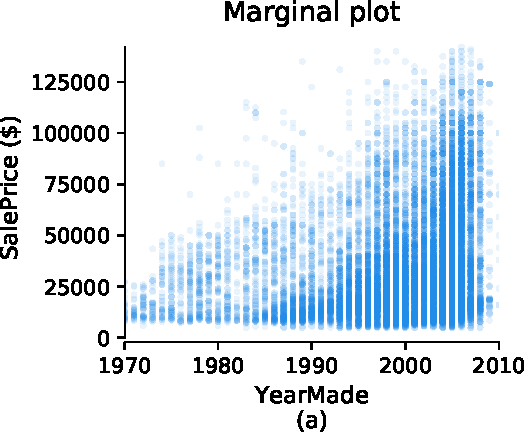
\includegraphics[scale=0.5]{images/bulldozer-YearMade-marginal.pdf}~~
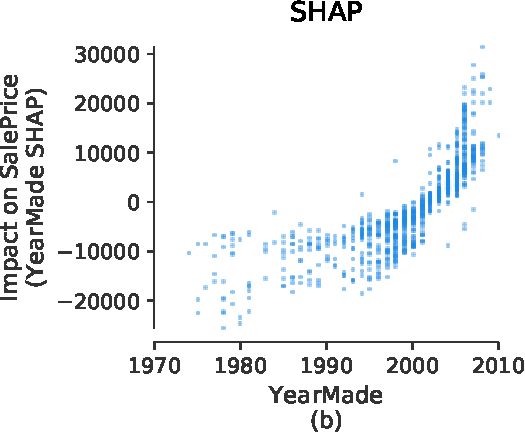
\includegraphics[scale=0.5]{images/bulldozer-YearMade-shap.pdf}~~
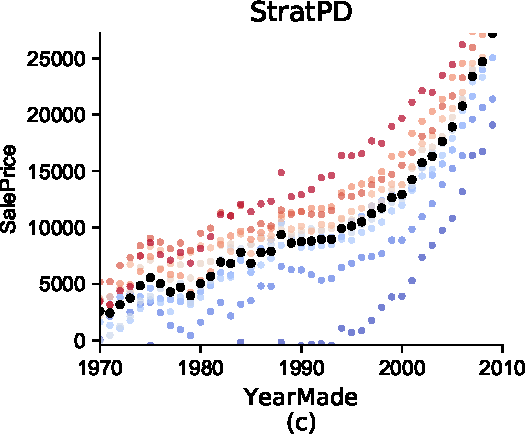
\includegraphics[scale=0.5]{images/bulldozer-YearMade-stratpd.pdf}
\caption{\small Bulldozer age vs SalePrice, as drawn by SHAP library and StratPD. 1000 SHAP values, 20k samples for stratpd}
\label{fig:shap-stratpd-YearMade}
\end{center}
\end{figure}

\section{Experimental results}\label{sec:experiments}

\todo{an experiment where we show insensitive to noise column and any other codependent ones that are thrown in but don't affect y}

\todo{maybe show the linear 1 1 1 codependence example}

\todo{what about outlier example}

\todo{show impact vs importance}

\todo{RF vs GBM}

\todo{stability is valuable. users would not trust results that changed significantly for small data set changes. show our error bars from bootstrapping and say we can do p-values.}

\todo{bulldozer: YearMade ignores too much with stratpd, use catstrat}

Even with domain expertise, humans are unreliable estimates of feature importance. Otherwise, we would need feature important mechanisms. Comparing the quality of feature importance methods is then a challenge. The simplest approach is to compare methods on synthetic data for which the answer is clear, such as the quadratic in \ref{eq:quad}.

For real data sets, we can train a predictive model on the most important $k$ features and compare prediction error. The importance method that accurately identifies the most impactful features without getting confused by codependent features, should yield lower production errors for a given $k$.   This mirrors how one would use it for model feature selection.
 
The best feature importance method ranks features by their independent contributions to $y$, without getting confused by codependent features. The most important single feature as reported by two importance methods can be used to train a model and measure a prediction metric.
 
{\bf Definition 3} The {\em top-k} fitness measure trains a suitable model on the  most important $k$ features as reported by two or more importance methods then compares prediction metrics. Actually p246 \citep{liu-fs} has an example of this.

even if recommendations are identified by their isolated contribution, the model is still taking the combination into consideration when fitting and hence the marginal errors are not necessarily reduced specifically because of the added feature at number $k$.

Get a baseline \figref{fig:baseline}.

\begin{figure}
\centering
\begin{subfigure}{.24\textwidth}
    \centering
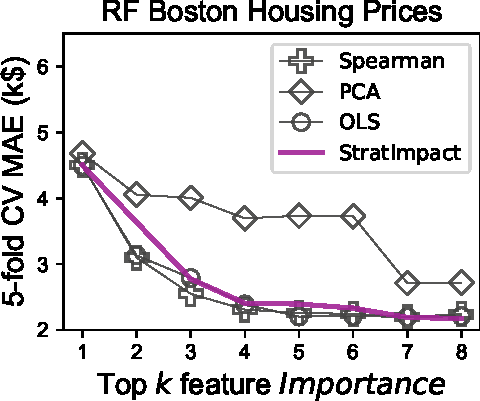
\includegraphics[scale=0.51]{images/boston-topk-baseline-Importance.pdf}
\subcaption{\footnotesize foo}
\end{subfigure}%
\hfill
\begin{subfigure}{.24\textwidth}
    \centering
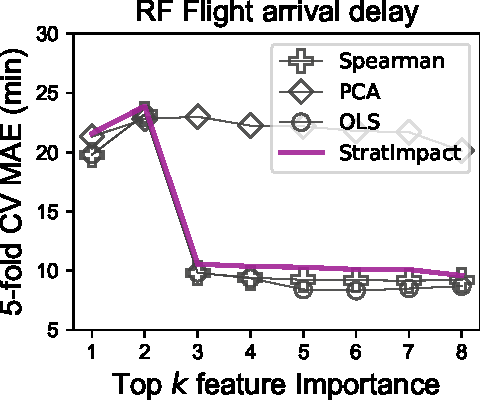
\includegraphics[scale=0.53]{images/flights-topk-baseline-Importance.pdf}
\subcaption{\footnotesize foo}
\end{subfigure}
\hfill
\begin{subfigure}{.24\textwidth}
    \centering
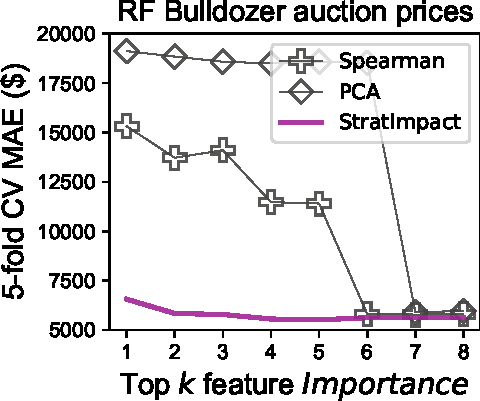
\includegraphics[scale=0.53]{images/bulldozer-topk-baseline-Importance.pdf}
\subcaption{\footnotesize foo}
\end{subfigure}
\hfill
\begin{subfigure}{.24\textwidth}
    \centering
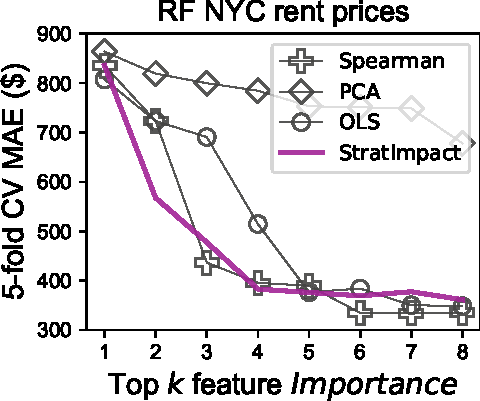
\includegraphics[scale=0.44]{images/rent-topk-baseline-Importance.pdf}
\subcaption{\footnotesize foo}
\end{subfigure}
\caption{Whew}
\label{fig:baseline}
\end{figure}

Model-based methods have all the advantages in these experiments.

In \figref{fig:features}, we

Then see \figref{fig:topk}

\begin{figure}
\centering
\begin{subfigure}{.24\textwidth}
    \centering
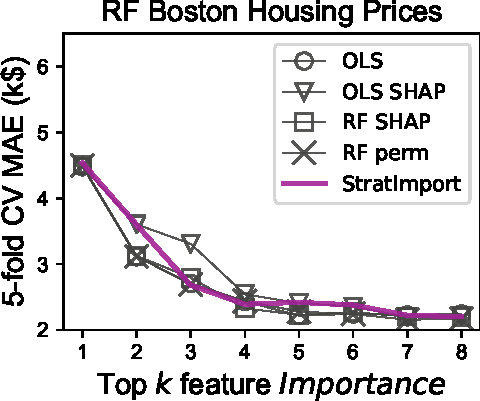
\includegraphics[scale=0.48]{images/boston-topk-RF-Importance.pdf}
\subcaption{\footnotesize foo}
\end{subfigure}%
\hfill
\begin{subfigure}{.23\textwidth}
    \centering
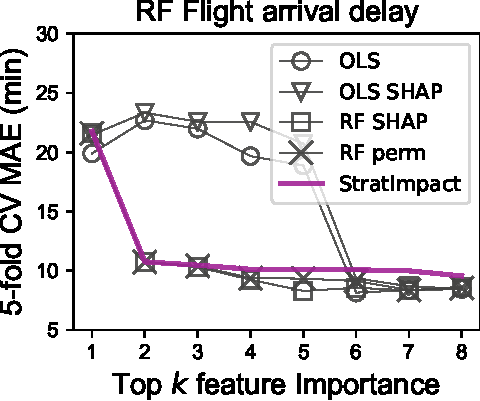
\includegraphics[scale=0.48]{images/flights-topk-RF-Importance.pdf}
\subcaption{\footnotesize foo}
\end{subfigure}
\hfill
\begin{subfigure}{.25\textwidth}
    \centering
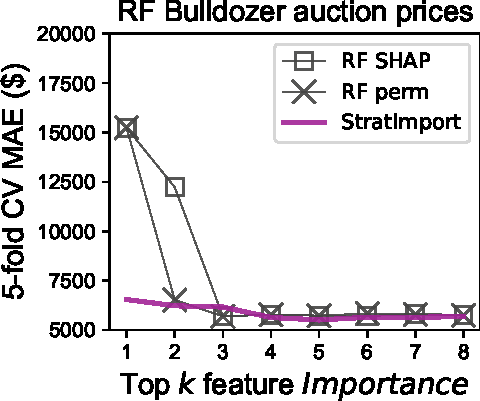
\includegraphics[scale=0.5]{images/bulldozer-topk-RF-Importance.pdf}
\subcaption{\footnotesize fff}
\end{subfigure}%
\hfill
\begin{subfigure}{.2\textwidth}
    \centering
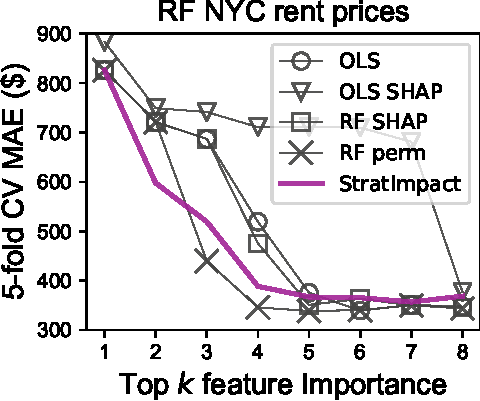
\includegraphics[scale=0.5]{images/rent-topk-RF-Importance.pdf}
\subcaption{\footnotesize foo}
\end{subfigure}
\caption[short]{Features from RF model, tested on RF}
\label{fig:topk}
\end{figure}

Show impact vs import in \figref{fig:topk-impact}

\begin{figure}
\centering
\begin{subfigure}{.24\textwidth}
    \centering
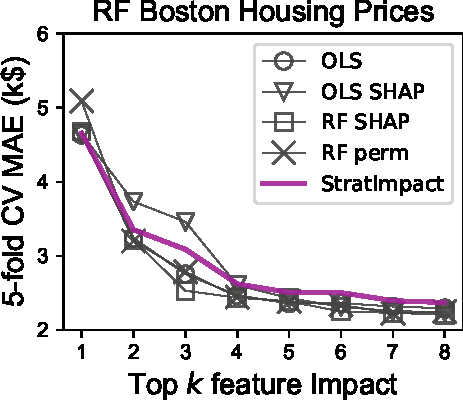
\includegraphics[scale=0.48]{images/boston-topk-RF-Impact.pdf}
\subcaption{\footnotesize foo}
\end{subfigure}%
\hfill
\begin{subfigure}{.23\textwidth}
    \centering
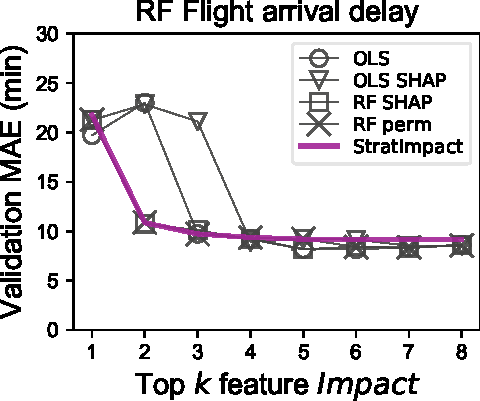
\includegraphics[scale=0.48]{images/flights-topk-RF-Impact.pdf}
\subcaption{\footnotesize foo}
\end{subfigure}
\hfill
\begin{subfigure}{.25\textwidth}
    \centering
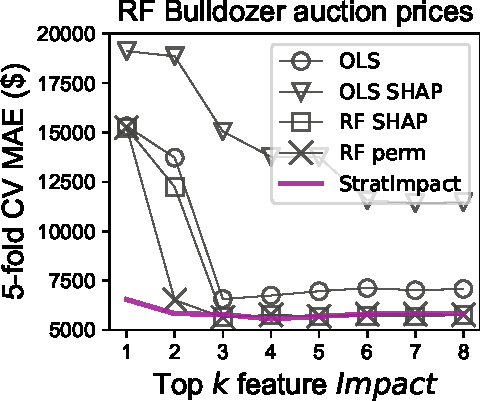
\includegraphics[scale=0.5]{images/bulldozer-topk-RF-Impact.pdf}
\subcaption{\footnotesize sometimes we get age as first feature which is ok but not the amazing ModelID, clearly best. 100 = 81/100 ModelID is top and 19/100 age is top}
\end{subfigure}%
\hfill
\begin{subfigure}{.2\textwidth}
    \centering
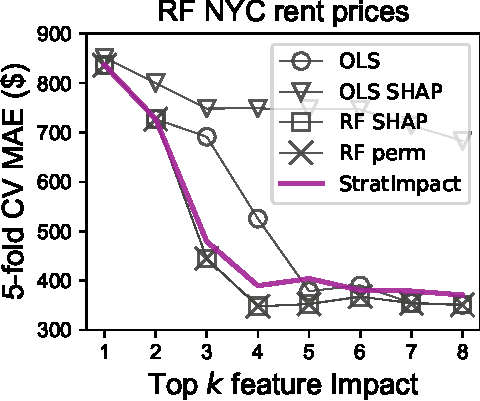
\includegraphics[scale=0.5]{images/rent-topk-RF-Impact.pdf}
\subcaption{\footnotesize foo}
\end{subfigure}
\caption[short]{Features from RF model, tested on RF}
\label{fig:topk-impact}
\end{figure}

Show \figref{fig:lasso}

\begin{figure}[htbp]
\begin{center}
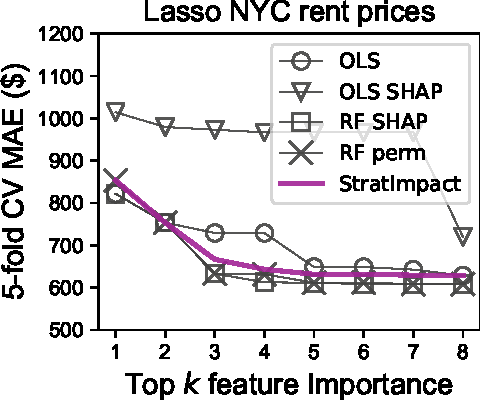
\includegraphics[scale=0.65]{images/rent-topk-Lasso-Importance.pdf}
\captionof{figure}{Lasso model}
\label{fig:lasso}
\end{center}
\end{figure}


\begin{figure}
\centering
\begin{subfigure}{.24\textwidth}
    \centering
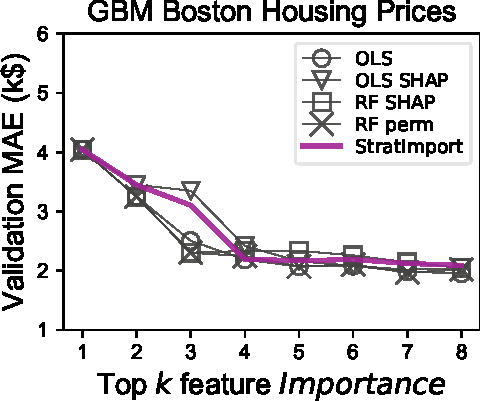
\includegraphics[scale=0.48]{images/boston-topk-GBM-Importance.pdf}
\subcaption{\footnotesize foo}
\end{subfigure}%
\hfill
\begin{subfigure}{.23\textwidth}
    \centering
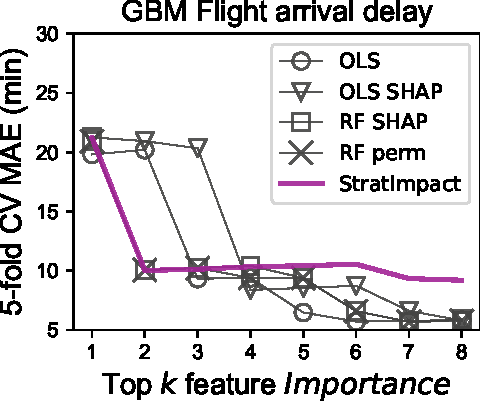
\includegraphics[scale=0.48]{images/flights-topk-GBM-Importance.pdf}
\subcaption{\footnotesize foo}
\end{subfigure}
\hfill
\begin{subfigure}{.25\textwidth}
    \centering
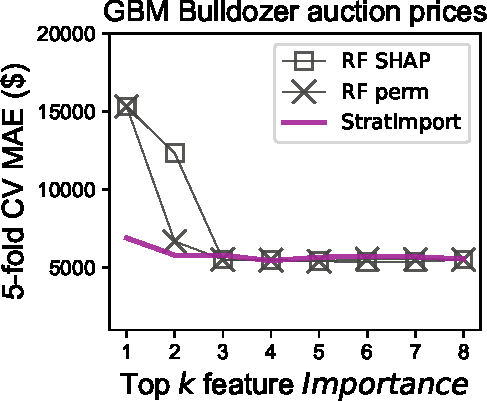
\includegraphics[scale=0.5]{images/bulldozer-topk-GBM-Importance.pdf}
\subcaption{\footnotesize abc}
\end{subfigure}%
\hfill
\begin{subfigure}{.2\textwidth}
    \centering
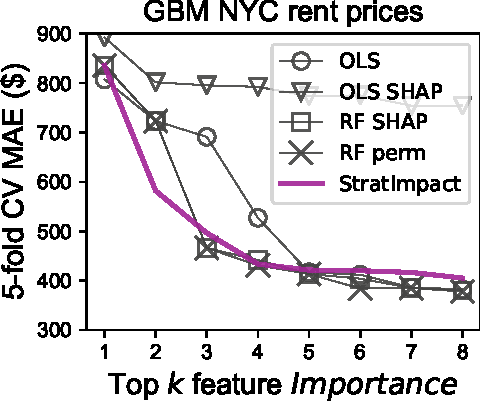
\includegraphics[scale=0.5]{images/rent-topk-GBM-Importance.pdf}
\subcaption{\footnotesize foo}
\end{subfigure}
\caption[short]{Features from RF model, tested on gradient boosting machine}
\label{fig:topk}
\end{figure}


\begin{figure}
\centering
\begin{subfigure}{1\textwidth}
    \centering
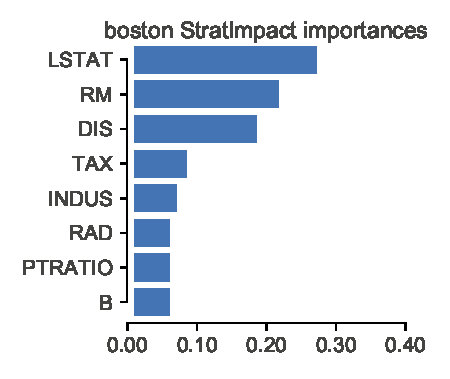
\includegraphics[scale=0.6]{images/boston-features.pdf}
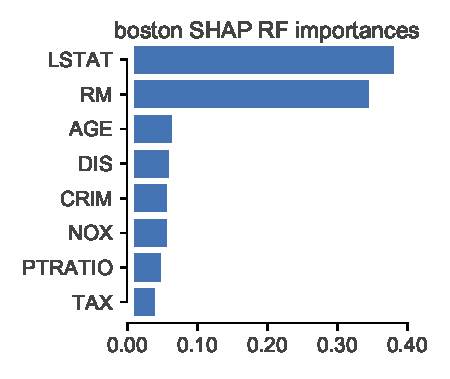
\includegraphics[scale=0.6]{images/boston-features-shap-rf.pdf}
\vspace{-2mm}\subcaption{\footnotesize Note LSTAT/RM order is diff than in original figure as their is high variance}\vspace{3mm}
\end{subfigure}%
\hfill
\begin{subfigure}{1\textwidth}
    \centering
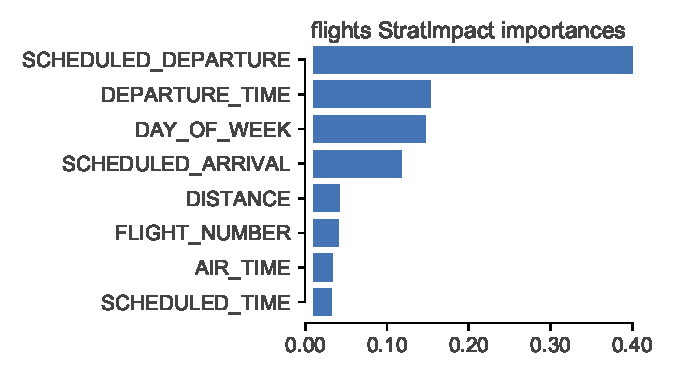
\includegraphics[scale=0.6]{images/flights-features.pdf}
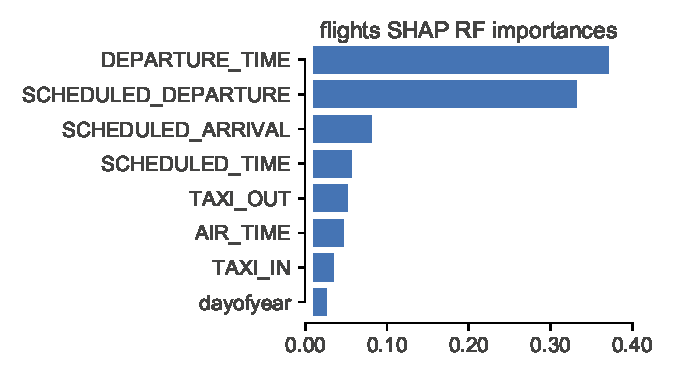
\includegraphics[scale=0.6]{images/flights-features-shap-rf.pdf}
\vspace{-2mm}\subcaption{\footnotesize 5.8M records}\vspace{3mm}
\end{subfigure}
\hfill
\begin{subfigure}{1\textwidth}
    \centering
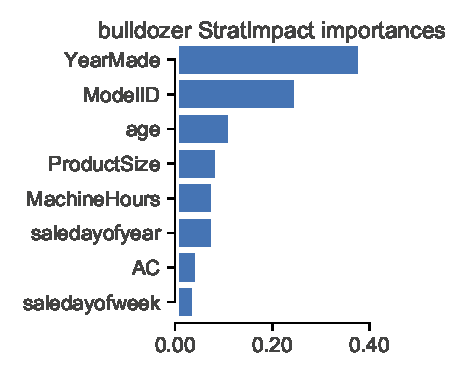
\includegraphics[scale=0.6]{images/bulldozer-features.pdf}
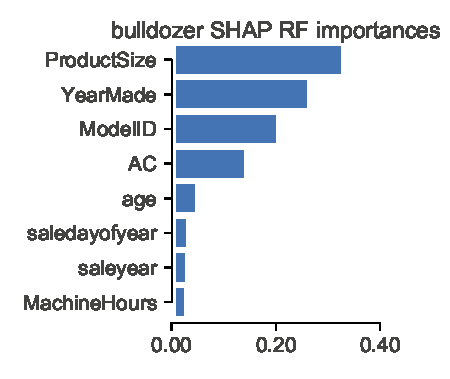
\includegraphics[scale=0.6]{images/bulldozer-features-shap-rf.pdf}
\vspace{-2mm}\subcaption{\footnotesize foo}\vspace{3mm}
\end{subfigure}%
\hfill
\begin{subfigure}{1\textwidth}
    \centering
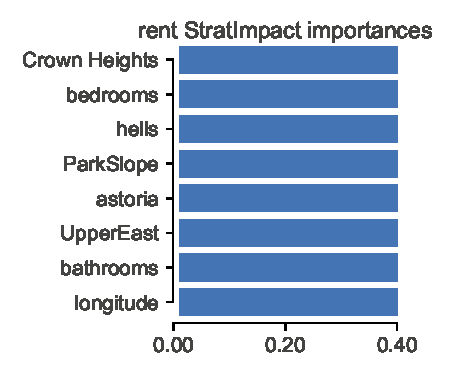
\includegraphics[scale=0.6]{images/rent-features.pdf}
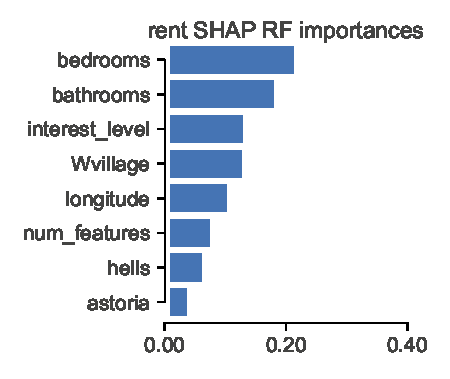
\includegraphics[scale=0.6]{images/rent-features-shap-rf.pdf}
\vspace{-2mm}\subcaption{\footnotesize foo}\vspace{3mm}
\end{subfigure}
\caption[short]{blorttttt}
\label{fig:features}
\end{figure}

Consider the recommendations from OLS SHAP used in a random forest. In general, they are not good recommendations. This demonstrates that the rank of features is highly dependent upon the model used to get those recommendations. In some cases, plain OLS recommendations fitted to RF beats the recommendations from OLS SHAP fitted to the RF.

Do an experiment that compares PCA and Spearman's R against StratImpact.

performance. with lots of outliers, choosing a small subset for shap is a bad idea so this is a real problem. linear and boosted trees are efficient but RF are not and I wouldn't consider anything using the general explainer.

There are issues surrounding how many explanatory samples you can use. 300 even run a couple of times is not enough to sample 5.8M records.

\todo{We need min samples per x to avoid left edge issues as they skew entire pdp, which severely skews mass AUC.}

\todo{explain cat mechanism and how there is no left/right edge so no evidence used to weight AUC.}
 
\section{foo}

 what is the definition: loosely as which are most predictive

The variance of the importances derived from the random forest is high, SHAP has specialized ``explainers'' for linear and tree-based models for performance reasons, but relies on the general method to explain support vector machines. , but the results are subject to the variance of the internal model parameters.  Ideally, feature importances would not change from run to run on the same data set using the same technique.

\section{Discussion and future work}

We deal with all possible combinations for codependency's because of the nature of the partial dependence mechanism.

features important in one model are not exportable to another which also means that they're less likely to be useful for business insight.
 
For business insight purposes, practitioners often favor direct data analysis, but to perform machine learning model feature selection, practitioners strongly favor model-based techniques. The idea being that business insight should flow directly from the data without peering through a (possibly unneeded) predictive model.  Similarly, it stands to reason that computing feature importances using the intended predictive model would provide the most useful ranking.

Our experience is that model analysis techniques dominate in practice, even for business insight purposes. Part of this is due to the prevalence of machine learning model usage but is also because we conflate predictive with important.  Predictiveness is sometimes a function of the model choice, however, rather than the inherent importance of the feature. For example, there could be a complex but one-to-one relationship between a variable and the response variable. A model unable to capture that relationship would show it as unpredictive, which is easy to confuse with unimportant.  On the other hand, important or not, tuning a model using what it considers predictive is useful in practice. Consequently, it might make sense to continue the bifurcation between data analysis for business insight and model analysis for model feature selection.

research should now focus on getting more accurate partial dependence approximations.

must define for classification

\vskip 0.2in
\bibliography{pdimp}
\end{document}